\documentclass[12pt, letterpaper]{article}

% Shared preamble (palette, macros, geometry)
\input{../../../Preambles/header.tex}

\usepackage[round, sort&compress, authoryear]{natbib}
\bibliographystyle{aer}
\usepackage{setspace}
\onehalfspacing
\usepackage[margin=1.1in]{geometry}

\title{Keeping the House in the Family:\\ Non-Market Transfers and the Supply of American Homes\thanks{Saani Rawat, Marquette University. Email: saani.rawat@marquette.edu. CoreLogic deed and property records were obtained through the University of Cincinnati's academic license. We thank \dots\ for helpful comments. All errors are our own.}}
\author{Saani Rawat\\Marquette University}
\date{\today\\\vspace{4pt}\textit{Preliminary and incomplete --- please do not cite without permission}}

\begin{document}
\maketitle

\begin{abstract}
\noindent A large share of American homes change hands without a market.
Using 144 million deed records covering the universe of recorded residential
transfers from 2007 to 2023, this paper provides the first
national deeds-based accounting of intra-family housing transfers. After
stripping out trust retitling and same-person co-owner changes, families
moved nearly 20 million homes between relatives over this period---one
family transfer for every 3.6 market sales---almost always at a recorded
price of zero. These transfers are not a staging step toward sale: three in
five family-transferred homes have not sold on the open market a decade
later. A simple model shows that when heirs inherit a below-market
property-tax assessment along with the house, families keep homes that the
market values more. California's Proposition~19, which abruptly ended
assessment inheritance for non-occupant heirs in February 2021, provides the
experiment. Family transfers surged 31 percent above counterfactual in the
four months before the deadline---February, normally the quietest month,
became the busiest in the series---and then fell to a new, persistently
lower level: 35 percent below baseline by 2022--2023, 23 percent net of a
market-sale placebo (placebo-state permutation $p \approx 0.10$ and $0.18$),
a missing flow of roughly 58,000 deeds per year, commensurate with the
60,000--80,000 tax-excluded inherited properties the state's fiscal analyst
counted annually under the old regime. The homes that exited the family
channel have not yet surfaced as estate sales, indicating deferred
successions rather than immediate listings. Our results suggest that family transfers are not outside the housing market but one of its allocation mechanisms, and property-tax rules can shift scarce homes from price-based matching to lineage-based retention. \\
\textbf{JEL classification:} R21, R31, H22, D64 \\
\textbf{Keywords:} housing supply, intergenerational transfers, bequests, property taxes, Proposition 19
\end{abstract}

\clearpage

\section{Introduction}\label{sec:intro}

The housing market that economists study is the one with prices. Sales are
recorded, indexed, and aggregated. Turnover, liquidity, and supply are all
defined over transactions in which a willing buyer pays a willing seller.
But county deed records reveal a second, often understudied, parallel circulation of houses that
satisfies none of these definitions: family transfers.
Between 2007 and 2023, American families
recorded nearly 20 million transfers of residential property between
relatives---a mother quitclaiming a bungalow to her son, siblings dividing a
deceased parent's house, a grandfather deeding a rental to a grandchild. For
every 3.6 homes sold on the open market, one moved through this family
channel. Almost none of these transfers involved money: nine in ten record
no price at all. None involved a listing, an appraisal, or a price signal.
The largest asset most households ever own is routinely allocated not by the
market but by the family---and the deed records that document this
allocation have gone largely unexamined.

This paper makes three contributions. First, it measures the family channel. We
construct a taxonomy of all 144 million recorded residential deed events in
the United States from 2007 to 2023, separating arm's-length market sales
from inter-person family transfers, trust self-transfers, same-person
co-owner retitling, and other non-market conveyances, using the names on the
deeds themselves to distinguish a true intergenerational transfer from a
household retitling its own home into a revocable trust or adding a spouse
to a title. The family channel is large, stable, and systematically
patterned: family transfers are relatively more common for older houses, for
parcels with senior tax exemptions, and at the bottom of the value
distribution---the signature of a bequest pipeline, not of disguised sales.
Its geography is equally telling. The family share is highest in California,
where one family transfer is recorded for every 1.6 market sales---2.3 times
the national ratio---and where, not coincidentally, the property-tax code
made dynastic holding most valuable.

Second, it follows the houses. Because each parcel carries a permanent
identifier, we can ask what happens to a home after it passes within a family.
The answer is bimodal. A minority of family transfers are settlement
waypoints: among cross-surname family conveyances---the class that includes
estate distributions---one in ten reaches the open market within a year, as
heirs take title and cash out. But the majority are destinations. Ten years
after a same-surname family transfer, 62 percent of homes have still never
sold on the open market, a retention rate exceeding that of homes bought on
the market by their owner-occupants and investors combined. Houses that enter
the family channel mostly stay there.

Third, and centrally, it shows that tax policy shapes this allocation. The
mechanism is easiest to see in California. Proposition~13 (1978) ties each
parcel's assessed value to its acquisition price; Propositions~58 (1986) and
193 (1996) let parents pass that assessed value to children along with the
house. An heir could thereby inherit a Pasadena house worth \$1.5 million and
pay property taxes on a 1980s basis---a subsidy available only if the family
\emph{kept} the house. The state's Legislative Analyst's Office estimated
that 60,000 to 80,000 inherited properties escaped reassessment each year and
observed, presciently, that the exclusion ``appears to be encouraging
children to hold on to their parents' homes to use as rentals or other
purposes instead of putting them on the for sale market''
\citep{lao2017inheritance}. Proposition~19, passed in November 2020 and
effective February 16, 2021, abruptly ended this regime: the exclusion now
survives only when the child occupies the home as a principal residence, and
only up to a value cap; for rentals and second homes it vanished entirely
\citep{boe2025prop19}.

The deeds record the response with unusual clarity. In the four months
between passage and the deadline, California families rushed to lock in the
old basis: family transfers ran 31 percent---29,000 deeds---above a
counterfactual built from California's own seasonal pattern and the rest of
the country's contemporaneous growth. After the deadline they collapsed to a
persistently lower level. In the 2022--2023 steady state, family transfers
were 35 percent below their pre-reform baseline relative to other states;
netting out California's contemporaneous slump in market sales leaves a 23
percent decline, roughly 58,000 transfers per year. Because California is a
single treated state, we assess these estimates against a placebo
distribution in which every other state is assigned the treatment in turn;
California's decline ranks fifth of fifty-one ($p \approx 0.10$), with the
larger placebo declines concentrated in its boom-and-bust Western neighbors.
The timing evidence is harder to mimic: within California, family transfers
were flat relative to 2019 through 2021 and then dropped 28 percent in 2022
and 36 percent in 2023. The missing flow is commensurate with the
Legislative Analyst's count of 60,000--80,000 tax-favored inherited
properties per year: the reform did not trim the family channel at the
margin so much as excise its tax-motivated core.

What happened to the homes that no longer pass between relatives? A simple
model of the heir's keep-or-sell decision makes the prediction precise, and
subtle. When the tax wedge disappears, the heirs who switch behavior are
those who valued the house \emph{less} than the market did and kept it only
for the inherited tax basis---the marginal landlords. These homes need never
generate a family deed at all: the succession can simply end in an estate
sale. The family transfers that survive are selected---heirs who genuinely
want the house, disproportionately to live in it---so the model predicts
that post-reform family transfers should show a \emph{lower} subsequent
market-sale hazard, not because supply was not released but because the
release happens upstream, in transfers that no longer occur. The conditional
margins move in the predicted directions but are statistically
unremarkable; the volume margin is where the houses are. The natural next
question---do the missing homes surface as estate sales?---gets a clean
answer in the data: not yet. Market sales by estate and trust sellers in
California track other states through 2023. The transfers the reform
eliminated were largely inter-vivos deeds executed years before death; the
successions they anticipated have not yet occurred, and when they do, the
homes will face market-value reassessment in the hands of any non-occupant
heir. The reform's supply effect is real but deferred---an unusually clean
prediction for future data to test.

These findings connect three literatures that have largely run on separate
tracks. The economics of bequests---from strategic motives
\citep{bernheimshleifersummers1985bequest} to inter-vivos timing
\citep{mcgarry1999intervivos} to estate-tax planning \citep{kopczuk2007bequest}
and the macroeconomic return of inheritance \citep{piketty2011inheritance}---
has documented how wealth passes between generations, but in data where a
house is a dollar amount, not a parcel with an address and a subsequent
history. Housing wealth is the modal bequest and a central channel of
intergenerational wealth correlation \citep{charleshurst2003wealth}; this
paper supplies the asset-level record of how it moves. The lock-in
literature shows that property-tax institutions and financing terms anchor
owners in place---Proposition~13 lengthened California tenures
\citep{wasiwhite2005prop13}, assessment portability releases older movers
\citep{ferreira2010takeit}, low mortgage rates immobilize borrowers
\citep{fonsecaliu2024lockin}, and property-tax design shapes allocation
generally \citep{covenetal2024proptax}---but its unit of observation is the
living owner; this paper shows the lock survives death. And the
transaction-tax literature \citep{kopczukmunroe2015mansion,
slemrodwebershan2017dc, bestkleven2018notches, hilberlyytikainen2017transfer}
establishes that property transactions respond sharply to tax notches through
timing and volume; the Proposition~19 deadline generates the same anticipation
dynamics in transfers that have no price at all. Closest in spirit, the
misallocation argument descends from \citet{glaeserluttmer2003rentcontrol}:
when a scarce asset is allocated by queue---or here, by
blood---rather than by willingness to pay, the loss is not a transfer but
forgone surplus, and the houses withheld from the market are disproportionately
the older, cheaper stock through which housing filters down to lower-income
buyers \citep{rosenthal2014filtering}. To our knowledge, no prior academic
study provides a national, deeds-microdata accounting of intra-family housing
transfers or a causal evaluation of Proposition~19's inheritance provisions;
the nearest antecedents are an industry tabulation of inheritance deeds
\citep{delventhal2026inherited}, measurements of the heirs'-property subset
\citep{dobbsgaither2023heirs, burnettwm2025heirs}, and the Legislative
Analyst's own assessment-roll counts \citep{lao2017inheritance}.

Two scope conditions discipline the welfare reading. First, family transfers
are not waste; they carry sentimental value, insure family members, and
economize on transaction costs, and when the heir values the home most, the
family allocation is also the efficient one. The problem is the wedge: a tax
code that pays heirs to hold homes they value below the market price converts
a private gift into a social misallocation, larger where housing is scarcest.
Second, the Proposition~19 estimates measure the response of recorded
transfers in a single---if largest---state, whose acquisition-value assessment
made the wedge uniquely large; the national counterfactual in
Section~\ref{sec:magnitudes} is correspondingly framed as bounds.

The paper proceeds as follows. Section~\ref{sec:data} describes the deeds
and the taxonomy. Section~\ref{sec:facts} establishes the national facts.
Section~\ref{sec:lock} follows homes after transfer. Section~\ref{sec:framework}
presents the model. Section~\ref{sec:prop19} analyzes Proposition~19.
Section~\ref{sec:magnitudes} discusses magnitudes, and
Section~\ref{sec:conclusion} concludes.

\section{Data and the Anatomy of a Non-Market Transfer}\label{sec:data}

\subsection{Deeds}

Property records come from CoreLogic's Owner Transfer file
\citep{corelogic_data}, obtained through an academic license, which compiles
the universe of recorded deeds from county recorder offices. A deed is filed
whenever the legal ownership of a parcel changes---not only when a house is
sold. The same administrative trail that records a \$400,000 sale records a
mother quitclaiming her house to her son for nothing. Market-based datasets
(MLS listings, repeat-sales indices, mortgage originations) discard these
zero-price events by construction. Here they are the object of study.

The extract covers all fifty states and the District of Columbia. Coverage
is dense from 2007 through mid-2024; we use 2007--2023 for annual statistics
and treat 2024 as a partial year. Restricting to residential parcels and
deduplicating to one event per parcel per recording date yields 148.7 million
deed events (144.0 million in 2007--2023), linked through a permanent parcel
identifier that follows each house across successive owners.

\subsection{Classifying transfers}

CoreLogic flags each record with a primary category---arm's length or
not---and an interfamily indicator constructed from the recorder's
consideration, deed type, and name fields. We sharpen these flags into a
taxonomy using the buyer and seller names on the deed:

\begin{enumerate}
  \item \textbf{Market sale}: arm's-length category, recorded price of at
        least \$10,000, not flagged interfamily (71.1 million events,
        2007--2023).
  \item \textbf{Same-person retitle}: the named principal is the same person
        on both sides of the deed---an owner adding or removing a co-owner,
        typically at marriage, divorce, or refinancing (7.1 million). No
        transfer between people occurs, so these are tracked separately and
        never counted as family transfers.
  \item \textbf{Family transfer, same surname}: flagged interfamily, buyer
        and seller sharing a surname but not the same person, no trust
        involved (13.6 million). This is the conservative measure of
        inter-person family transfers---it misses, for example, transfers to
        a married daughter who changed her name, so it bounds the channel
        from below.
  \item \textbf{Family transfer, other}: flagged interfamily without a
        surname match---cross-surname relatives and in-laws---plus
        estate/executor deeds (6.1 million).
  \item \textbf{Trust self-transfer}: a trust appears on either side of the
        deed (12.1 million). The modal event is estate planning---a household
        retitling its own home into a revocable trust. Control does not
        change hands; tracked separately, never counted as family transfers.
  \item \textbf{Other non-arm's-length}: the remainder---divorce divisions
        across surnames, title corrections, nominal-price conveyances, and
        foreclosure-related instruments (34.0 million).
\end{enumerate}

Table~\ref{tab:taxonomy} validates the taxonomy on its observable
fingerprints, and the fingerprints are unambiguous. Family transfers look
nothing like sales: 90 percent of same-surname transfers record a price of
zero, against 0 percent of market sales (which require a price by
construction) and 65 percent of the residual non-arm's-length class; 40
percent travel by quitclaim deed---the instrument of gift---against 2 percent
of market sales. Where a price is recorded at all in a same-surname transfer,
the median is \$97,000, well under half the \$224,000 median market price:
family ``sales'' happen at family discounts. Corporate buyers, who take 10
percent of market purchases, are essentially absent from same-surname
transfers. These are gifts and bequests, not disguised transactions. One
note on probate: formal estate keywords (``estate of,'' executor,
administrator) rarely appear in the recorded name fields, so explicitly
labeled estate deeds are a small class; most succession conveyances travel as
ordinary interfamily deeds and are captured in the same-surname and
cross-surname classes.

\input{tables/T1_taxonomy.tex}

\section{The Parallel Housing Market: National Facts}\label{sec:facts}

\paragraph{Fact 1: For every 3.6 market sales, one home moves within a family.}
Table~\ref{tab:volumes} and Figure~\ref{fig:volumes} report annual volumes.
Between 0.9 and 1.6 million homes pass between family members every year
(same-surname plus other interfamily), against 3.0 to 5.8 million market
sales: a family:market ratio between 0.25 and 0.34 in every year of the
sample, with a 2007--2023 aggregate of 0.28. The conservative same-surname
series alone runs 0.7 to 1.0 million per year. The channel is not a
recession artifact: the ratio was as high in the 2009 bust (0.29) as in the
2021 boom (0.28). And the count is deliberately strict---it excludes the 12.1
million trust self-transfers, 7.1 million same-person retitles, and 34.0
million other non-market conveyances; adding them, the deed traffic outside
the market rivals the market itself.\footnote{Restricting the denominator to
existing homes (excluding new-construction first sales) raises the aggregate
family:market ratio to 0.30. On a per-property rather than per-deed basis,
the 19.7 million family-transfer deeds cover 16.5 million distinct parcels
(1.19 deeds per parcel).}

\input{tables/T2_volumes.tex}

\begin{figure}[!t]
  \centering
  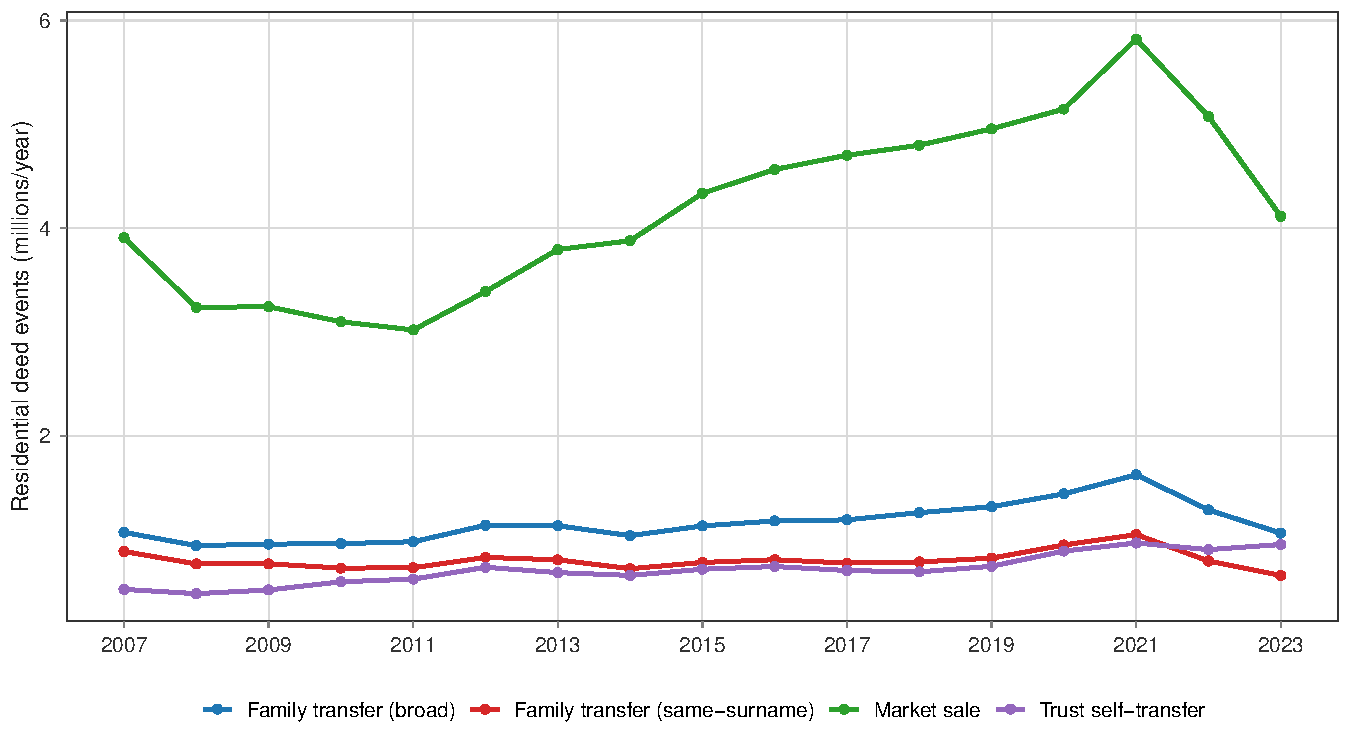
\includegraphics[width=0.92\linewidth]{figures/F1_volumes.pdf}
  \caption{Residential deed events by class, 2007--2023. Family transfer
  (broad) combines same-surname, other-interfamily, and estate/executor
  classes; trust self-transfers are shown separately.}
  \label{fig:volumes}
\end{figure}

\paragraph{Fact 2: The family channel rises where holding is tax-subsidized.}
Figure~\ref{fig:stateratio} ranks states by the family:market ratio over
2017--2023. California leads the nation at 0.61---one family transfer for
every 1.6 market sales, 2.3 times the pooled national ratio of 0.26---ahead
of Utah and Idaho (0.53). California is exactly where acquisition-value
assessment made the inherited tax basis most valuable, and it also accounts
for 38 percent of all trust self-transfers in the country (2.2 million over
seven years, more than its family transfers), the signature of an
estate-planning industry built around property-tax basis. Cross-state
correlations are not causal evidence---demography, land tenure, and recording
practice all differ---but the cross-section puts the tax-subsidy hypothesis
on the table, and Section~\ref{sec:prop19} tests it within California.

\begin{figure}[!t]
  \centering
  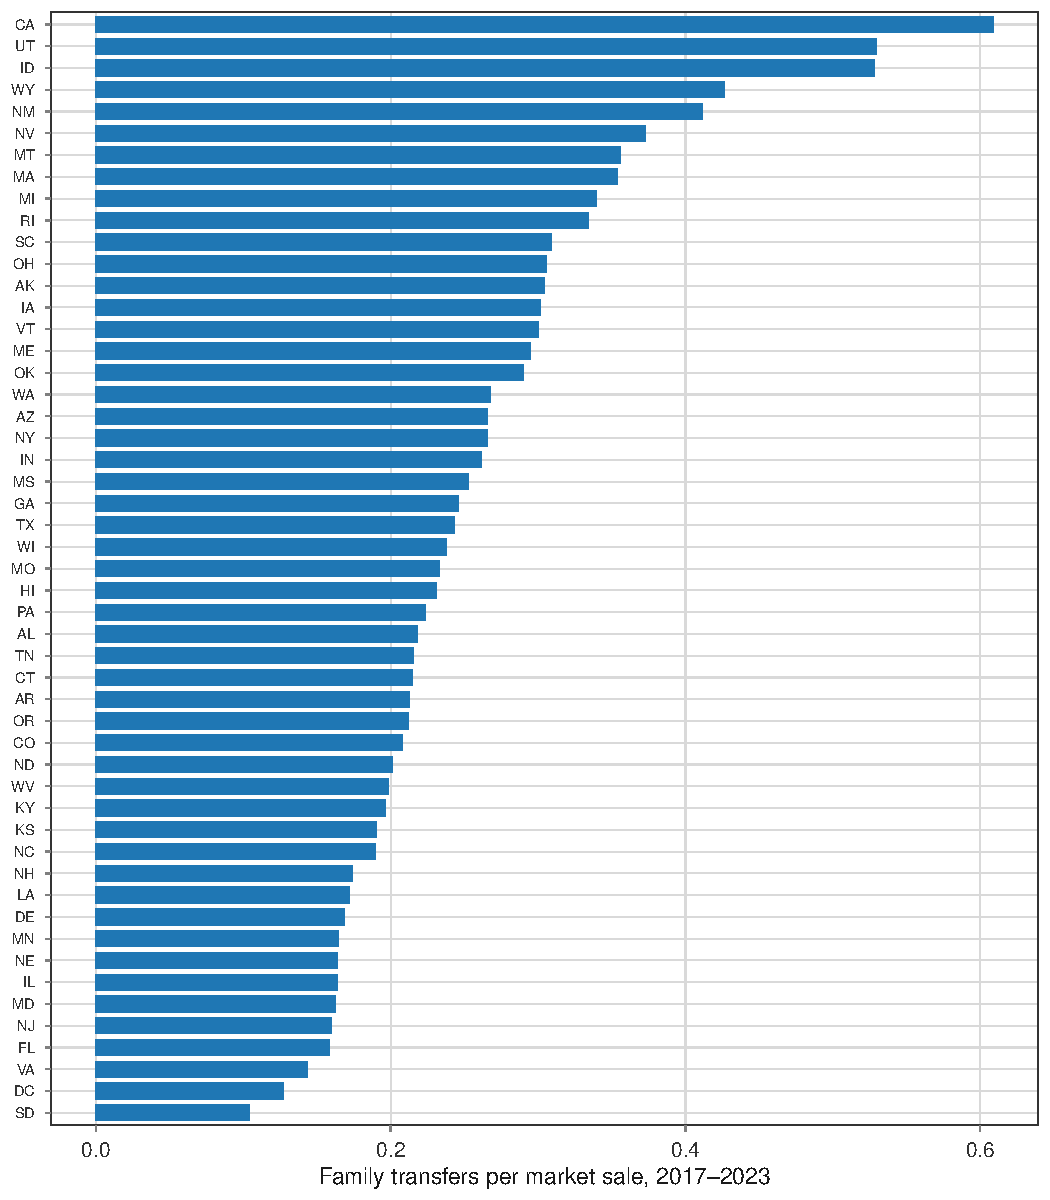
\includegraphics[width=0.78\linewidth]{figures/F2_state_ratio.pdf}
  \caption{Family transfers (broad) per market sale by state, 2017--2023.}
  \label{fig:stateratio}
\end{figure}

\paragraph{Fact 3: Family transfers carry the old housing stock.}
Linking deed events to property characteristics (61 percent of 2017--2023
events match the current assessment snapshot; Appendix~\ref{app:data}),
the family share of within-class traffic rises with structure age: family
transfers are 20 percent of combined family-plus-market events for houses
of ten to thirty years, 22 percent at thirty to fifty years, and 26 percent
at fifty to seventy-five years. The family share is higher on parcels with
senior tax exemptions (26 versus 22 percent)---the bequest pipeline made
visible---and declines monotonically across the within-state value
distribution, from 25 percent in the bottom quintile to 21 percent in the
top. The houses that families keep are disproportionately the older, cheaper
stock through which housing filters down to lower-income buyers
\citep{rosenthal2014filtering}.

\section{The Family Lock}\label{sec:lock}

What happens to a house after it enters the family channel? Because the
parcel identifier links successive deeds, every transfer event can be
followed to the property's next arm's-length market sale, if any. We take all
events in the 2008--2018 cohorts---guaranteeing at least 66 months of
follow-up before the June 2024 censoring date---and estimate Kaplan--Meier
survival to first market sale, separately by event class:
8.5 million same-surname family transfers, 3.4 million other family
transfers, 7.1 million trust self-transfers, 4.1 million same-person
retitles, and 42.1 million market purchases as the benchmark.

Table~\ref{tab:hazard} and Figure~\ref{fig:km} show two distinct family
destinies. The first is settlement: among cross-surname family
conveyances---the class containing estate distributions among multiple
heirs---10 percent reach the open market within twelve months and 15 percent
within twenty-four, roughly double the market-purchase benchmark (5 and 9
percent). For a substantial minority, the family deed is the
administrative final step before the house is sold.

The second destiny is the lock. Once a family-transferred home survives the
settlement window, it becomes more immobile than the housing stock at large.
Same-surname transfers start faster than market purchases (11.1 versus 8.9
percent sold within two years) but fall behind by year five (23.1 versus
23.7 percent) and keep falling behind: by year ten, 38 percent of
same-surname family homes have returned to the market against 42 percent of
market purchases. Conditional on passing the two-year settlement phase, 30
percent of family homes sell over the following eight years versus 36
percent of market purchases. The market-purchase benchmark, recall, includes
investors and flippers; family homes are stickier than all of it. Three in
five of the homes that passed between relatives in 2008--2018 had not sold
on the open market a decade later. The taxonomy passes an internal
falsification along the way: same-person retitles---title changes with no
transfer of control---track trust self-transfers almost exactly (9.1 versus
8.9 percent sold within two years), exactly as paperwork events should.

This is a descriptive fact, and selection is its content: families keep the
homes they receive. Four caveats discipline its reading. First, the
comparison pools states and cohorts; family transfers concentrate in older
homes and in low-turnover states, so part of the gap is composition (a
stratified version is planned for the next draft). Second, the two clocks
measure different objects: a market purchase starts a fresh tenure, while a
family deed often changes title without changing occupancy---a force that
should, if anything, \emph{raise} the family class's sale hazard, since
family deeds cluster near succession events. Third, some cross-surname
family homes cannot sell for title reasons (heirs' property), a lock of a
different kind \citep{dobbsgaither2023heirs}. Fourth, trust self-transfers
---pure retitling with no change of control---show survival close to the
same-surname class, a reminder that long-tenure households are exactly the
ones that do estate paperwork. Whether family retention reflects genuine
attachment or a tax wedge is therefore exactly what the cross-sectional data
cannot say---and what Proposition~19 can.

\input{tables/T3_hazard.tex}

\begin{figure}[!t]
  \centering
  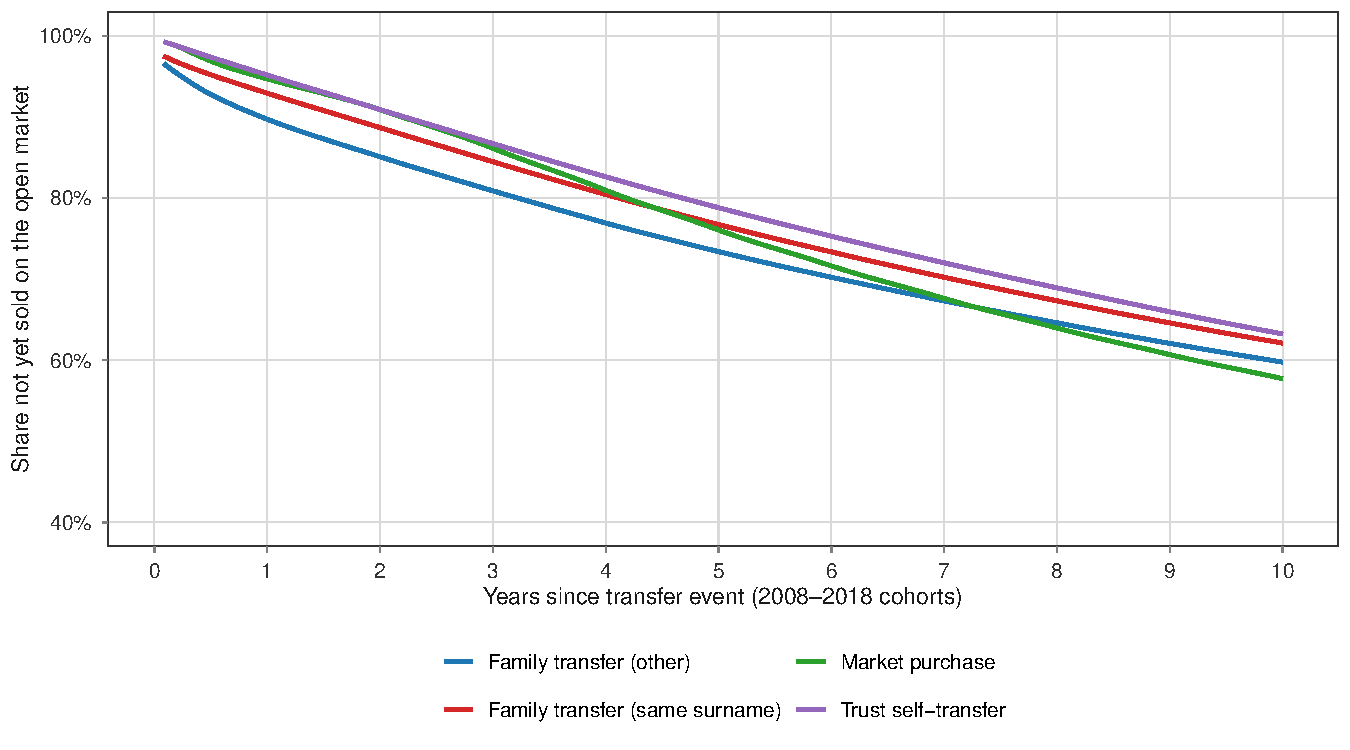
\includegraphics[width=0.92\linewidth]{figures/F3_km_curves.pdf}
  \caption{Kaplan--Meier survival to first open-market sale, 2008--2018
  event cohorts, censored June 2024. The estate/executor class
  (n=915) is omitted.}
  \label{fig:km}
\end{figure}

\section{A Simple Framework}\label{sec:framework}

A two-line model clarifies why tax institutions matter for whether inherited
homes reach the market, and organizes the California evidence.

A house yields a flow value $u_m$ to the marginal market buyer. With property
taxes levied at rate $t$ on assessed value---and assessments reset to price at
sale---the price capitalizes the tax burden in perpetuity:
\begin{equation}
  p \;=\; \frac{u_m}{r + t},
\end{equation}
where $r$ is the discount rate. Now consider an heir at the moment of
succession who values living in the house (or renting it out) at flow $u_h$.
If the family keeps the house, the heir pays taxes on assessed value $A$; if
it sells, it receives $p$. Keeping is optimal if and only if
\begin{equation}
  \frac{u_h - tA}{r} \;\ge\; p
  \quad\Longleftrightarrow\quad
  u_h \;\ge\; u_m - t\,(p - A).
  \label{eq:keep}
\end{equation}

Equation~\eqref{eq:keep} contains the paper's economics. If succession
triggers reassessment ($A = p$), the condition collapses to $u_h \ge u_m$:
the house stays in the family only when the heir genuinely values it more
than the market does, and the family channel is allocatively harmless. But if
the heir \emph{inherits the parent's assessment} ($A = A_0 < p$), the family
keeps the house whenever $u_h \ge u_m - t(p - A_0)$. Every heir with
$u_h \in [\,u_m - t(p - A_0),\; u_m)$ retains a house that the market values
more than she does. The wedge $t(p - A_0)$---the annual tax saving from
dynastic holding---is a price the tax code pays families to keep houses off
the market. In California, where acquisition-value assessment dates to 1978
and house prices have multiplied since, the wedge on a long-held home is
measured in thousands of dollars per year, forever.

The key observational subtlety is that the \emph{recorded family transfer is
itself the outcome of the keep-or-sell choice}. When the family keeps, the
county records a family deed; when it cashes out, the estate sells directly
to a market buyer and no family transfer ever appears. The deed is endogenous
to the tax regime. This shapes what an unanticipated removal of assessment
inheritance for non-occupant heirs---which is what Proposition~19 did in
February 2021---should do to each observable margin.

First, \emph{retiming}: because a transfer completed before the deadline
locks in $A_0$, families with latent transfer plans rush to record deeds
before the effective date, and recorded transfers collapse afterward
\citep[cf. the transaction-tax notch literature:][]{kopczukmunroe2015mansion,
slemrodwebershan2017dc, bestkleven2018notches}. Second, the \emph{extensive
margin}: with the wedge removed, every heir in
$[\,u_m - t(p - A_0),\; u_m)$ switches from keep to sell---these homes exit
the family channel entirely and flow to the market as estate sales. The
steady-state volume of family transfers falls by the mass of heirs in the
wedge; that volume decline \emph{is} the supply release. Third,
\emph{selection}: the family transfers that survive are those with
$u_h \ge u_m$---heirs who genuinely want the house, disproportionately
owner-occupants, whom the surviving (occupancy-conditional) exclusion still
favors. The model therefore predicts that post-reform family transfers should
show a \emph{lower} subsequent market-sale hazard and a lower
absentee-recipient share---not because the reform failed, but because the
marginal would-have-been-landlord heirs no longer take title at all.

\section{Proposition 19: Death, Taxes, and the Return of Homes to the Market}\label{sec:prop19}

\subsection{Institutional background}

Proposition~13 (1978) fixed each California parcel's assessed value at its
acquisition price, with growth capped at two percent per year; reassessment
to market value occurs only at a change in ownership. Proposition~58 (1986)
exempted parent-to-child transfers from this reassessment---for a principal
residence of unlimited value plus up to \$1 million of assessed value of
other property---and Proposition~193 (1996) extended the exemption to
grandparent-grandchild transfers. A child could therefore inherit not just a
house but its decades-old tax bill, and keep that tax bill while renting the
house out. The Legislative Analyst's Office estimated that 60,000 to 80,000
inherited properties escaped reassessment each year under this regime
\citep{lao2017inheritance}.

Proposition~19, passed by voters on November 3, 2020, narrowed the exclusion
sharply, effective February 16, 2021: it now applies only when the home was
the parent's principal residence \emph{and} the child makes it their own
principal residence within a year, and only up to the inherited taxable value
plus \$1 million (inflation-adjusted); the exclusion for rentals, vacation
homes, and other non-primary-residence property was eliminated, with a
carve-out for family farms \citep{boe2025prop19, lao2020prop19}. For a
non-occupant heir, the reform sets $A = p$ in equation~\eqref{eq:keep}.
County assessors reported a flood of parent-child filings ahead of the
deadline.\footnote{Sonoma County, for example, received roughly five times
its typical volume of parent-child exclusion filings in the weeks before the
February 15, 2021 deadline (North Bay Business Journal, February 2021); the
Los Angeles County assessor accumulated a multi-year backlog of roughly
20,000 claims (Los Angeles County Auditor-Controller, 2025).} The reform's
other arm---expanded portability of assessments for movers aged 55 and over,
effective April 1, 2021---affects market sales rather than family transfers;
the designs below either difference it out with a market-sale placebo or use
outcomes it does not touch.

Throughout this section, ``family transfers'' means the broad class
(same-surname, cross-surname, and estate/executor deeds), measured monthly by
state from the event panel; results including trust self-transfers are
reported as robustness.

\subsection{Retiming: the rush to beat the deadline}

Figure~\ref{fig:bunching} plots monthly California family transfers against a
transparent counterfactual: California's 2019 volume in the same calendar
month, scaled by the rest of the country's contemporaneous growth in family
transfers. The counterfactual thus inherits both California's seasonality and
every national shock---COVID disruption, the 2020--2021 housing boom, the
estate-planning surge.

\begin{figure}[!t]
  \centering
  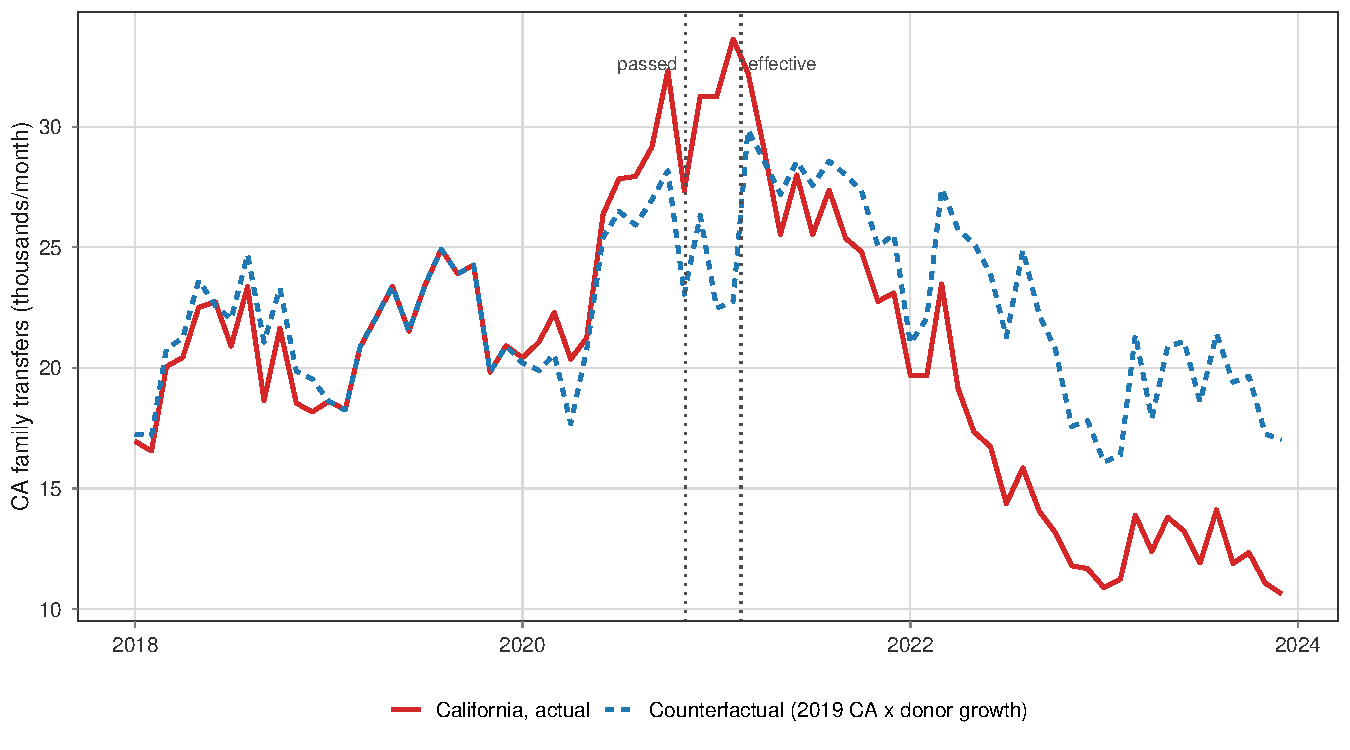
\includegraphics[width=0.92\linewidth]{figures/F4_prop19_bunching.pdf}
  \caption{California monthly family transfers (broad class) versus
  counterfactual (CA 2019 same-calendar-month volume $\times$ rest-of-US
  growth). Dotted lines: November 3, 2020 (passage) and February 16, 2021
  (parent-child provisions effective).}
  \label{fig:bunching}
\end{figure}

California tracks the counterfactual closely until November 2020. Between
passage and the deadline, the two series tear apart: from November 2020
through February 2021, actual family transfers total 123,486 against a
counterfactual of 94,620---an excess of 28,866 deeds, 31 percent above
counterfactual, crammed into four months. February 2021, ordinarily the
year's quietest month, became the busiest family-transfer month in the
2018--2023 California series. This is the anticipatory bunching that notch
designs recover for taxed market transactions \citep{bestkleven2018notches,
slemrodwebershan2017dc}, reproduced in transfers with no price: families
re-timed successions to bequeath a tax basis. Because the response is timed
to the day-specific deadline within a single state, no slow-moving
confounder---pandemic, migration, the housing cycle---can mimic it.

\subsection{The steady-state decline}

Retiming alone would imply a transitory post-deadline trough followed by
recovery. Instead, the gap persists and widens. From March 2021 through
December 2022, actual transfers run 85,000 below counterfactual (16
percent); by 2023, California family transfers (147,441) are 41 percent below
their 2018--2019 average (251,256)---while national volumes returned to
trend.

The difference-in-differences estimates in Table~\ref{tab:prop19} formalize
this. Using state-by-year counts for 2017--2019 versus 2022--2023 (the
transition years 2020--2021 are excluded as contaminated by anticipation and
retiming), with state and year fixed effects, log family transfers fall by
0.425 (s.e.\ 0.035) in California relative to other states---35 percent. The
placebo column shows log market sales falling 0.163 (15 percent) over the
same window, California's general post-rate-shock slump; netting it out
leaves a 23 percent decline specific to family transfers, roughly 58,000
transfers per year against the 2018--2019 base. Reclassification into trusts
cannot explain it: including trust self-transfers in the family aggregate
yields a decline of 0.241 log points (21 percent).

Two pieces of evidence address the design's limits. First, inference:
assigning the treatment to each donor state in turn, California's family
decline ranks fifth of fifty-one in absolute size (permutation
$p \approx 0.10$; for the placebo-netted estimate, $p \approx 0.18$), with
the largest placebo declines in Utah and Nevada---Western states sharing
California's boom-and-bust cycle, which is precisely what the market-sale
adjustment is for. Second, timing: an event-study version (California
$\times$ year, 2019 omitted) shows leads of $-0.03$ in 2018, $+0.06$ in
2020, and $-0.01$ in 2021---flat through the reform year, as the
pre-deadline rush and post-deadline collapse offset within 2021---followed
by $-0.33$ in 2022 and $-0.44$ in 2023 (28 and 36 percent below trend); the
one wobble is a $+0.15$ lead in 2017, so a conservative reading anchors the
baseline at 2018--2019, which yields almost the same post-period decline.
The missing annual flow, 58,000 deeds, sits inside the Legislative Analyst's
60,000--80,000 count of tax-excluded inherited properties per year: the
reform removed much of the tax-motivated component of the channel, and
little else.


\begin{table}[htbp]
   \caption{\label{tab:prop19} Proposition 19: volume, selection, and composition}
   \centering
   \scriptsize
   \begin{tabular}{lccccc}
      \tabularnewline \midrule \midrule
      Dependent Variables: & log(n\_fam) & log(n\_market) & \multicolumn{2}{c}{Sold within 24m} & Absentee share\\
      Model:                     & (1)            & (2)             & (3)      & (4)      & (5)\\
      \midrule
      \emph{Variables}\\
      CA $\times$ Post           & -0.4253        & -0.1626         & -0.0178  & -0.0104  & -0.0016\\
                                 & (0.0352)       & (0.0293)        & (0.0032) & (0.0019) & (0.0032)\\
      Synthetic-control rank     & 2/51 (p=0.039) &                 &          &          & \\
      Ann. placebo rank          & 5/51 (p=0.098) & 17/51 (p=0.333) &          &          & \\
      Fam. $-$ market log effect & -0.263         &                 &          &          & \\
      Monthly pre-fit rank       & 1/51 (p=0.020) &                 &          &          & \\
      \midrule
      \emph{Fixed-effects}\\
      State                      & Yes            & Yes             & Yes      & Yes      & Yes\\
      Year                       & Yes            & Yes             &          &          & \\
      Cohort month               &                &                 & Yes      & Yes      & Yes\\
      \midrule
      \emph{Fit statistics}\\
      Observations               & 255            & 255             & 1,836    & 1,836    & 1,836\\
      R$^2$                      & 0.98575        & 0.98961         & 0.84936  & 0.85147  & 0.90764\\
      \midrule \midrule
      \multicolumn{6}{l}{\emph{Clustered (State) standard-errors in parentheses}}\\
   \end{tabular}

   \par \raggedright
   Cols (1)-(2): state-year counts, 2017-2019 vs 2022-2023. Cols (3)-(5): cohort cells (2017m1-2018m12 vs 2021m7-2022m6), weighted by cell size. Clustered (state) SEs are shown only for scale. Single-treated-state inference for the steady-state volume decline is the synthetic-control in-space placebo (MSPE-ratio rank 2/51, $p=0.039$; Appendix Figure~\ref{fig:scm_mspe}); the annual and monthly-counterfactual placebo ranks are reported as transparent alternatives. The monthly pre-fit rank is the 2022-2023 California gap divided by its 2018m1-2020m10 counterfactual RMSPE, ranked against leave-one-out placebo states.
\end{table}


\subsection{Selection: who still keeps the house}

The model's third prediction concerns the transfers that survive. We take
family-transfer cohorts from two clean windows---January 2017 to December
2018 (pre) and July 2021 to June 2022 (post, after the retiming
turbulence)---and measure whether each transferred home reaches the open
market within 24 months, a window that closes before the June 2024 censor
for every cohort. Corporate recipients are excluded. The design compares
California to other states, cohort month by cohort month (state and
cohort-month fixed effects, weighted by cell size, clustered by state), with
the identical regression run on market \emph{purchases} as a placebo for
California-specific housing-cycle shocks; the triple-difference nets the two.

The raw numbers tell the story. Before the reform, California
family-transferred homes reached the market \emph{more} often than the
national average (16.1 versus 13.1 percent within 24 months)---California's
inherited-basis regime made even hold-motivated transfers cheap to unwind
later, and its hot market made selling attractive. After the reform,
California converges toward the national rate (12.3 versus 11.1 percent). In
the regression, the California post-reform effect is $-1.78$ percentage
points; the market-purchase placebo shows $-1.04$ points, and the
triple-difference is $-0.74$ points---a decline, as the selection logic
predicts, not a rise. But candor about inference is required here: the
triple-difference sits well within the placebo-state distribution
(permutation $p = 0.67$), and the absentee-recipient share is flat
($-0.2$ percentage points). The conditional margins move in the model's
direction and rule out the main alternative---had the missing transfers been
settlement deeds, the surviving pool would have shifted sharply toward
holders and the hazard would have fallen far more---but they do not carry
independent statistical weight. The volume margin is where the evidence
lives.

\subsection{Where are the missing homes? A direct test}\label{subsec:directtest}

If the heirs in the wedge now sell at succession instead of taking title,
the missing family deeds should eventually reappear as market sales by
estates and trusts. The deed names permit a direct test: market sales whose
seller carries an estate, executor, or trust designation. The answer, so
far, is that they have not reappeared. Estate- and trust-seller market sales
in California fall 8 percent relative to donor states between 2017--2019 and
2022--2023 (permutation $p = 0.71$); relative to California's overall market
slump they \emph{gain} 8 log points---their share of California market sales
rises from 28.4 to 31.9 percent---but similar share gains occur elsewhere
(permutation $p = 0.63$).

This null is informative rather than embarrassing, because it discriminates
between two readings of the volume decline. If the eliminated deeds had been
transfers of homes whose succession was imminent---parents recently deceased,
estates in settlement---the market should have received those homes within
the 2022--2023 window. It did not. The eliminated deeds were instead
predominantly \emph{inter-vivos} transfers, executed while the parent was
alive precisely to lock in the tax basis years or decades ahead of
succession; absent the tax motive, the parents simply keep title, and
nothing observable happens until they die. The reform's effect on market
supply is therefore real but deferred: every one of these postponed
successions now ends with reassessment at market value in the hands of any
non-occupant heir, and equation~\eqref{eq:keep} says more of those homes
will be sold when the time comes. The deeds data will eventually record
whether they are---a sharp, falsifiable prediction this paper leaves armed.

\subsection{Threats to identification}

California is a single treated state, so conventional
clustered standard errors understate uncertainty regardless of the number of control
states. Table~\ref{tab:prop19} reports them for
transparency. We also use placebo-state permutation for inference:
each donor state is assigned the treatment in turn, the design is
re-estimated, and California's coefficient is ranked in the resulting
distribution.

Five substantive threats to identification deserve mention.

\begin{itemize}
\item \emph{COVID and the 2020--2021
turbulence}: the bunching counterfactual absorbs national pandemic shocks by
construction (with the caveat that it is anchored to California's 2019
seasonal pattern, so its pre-period fit is validated out of sample only in
2018 and the first ten months of 2020); the steady-state DiD excludes
2020--2021 entirely; and the placebo run on market sales nets out
California-specific cycle effects.
\item \emph{Differential mortality and
migration}: family transfers are driven by deaths and aging, and California's
cumulative COVID mortality was below the national average while elevated
mortality elsewhere pulled successions forward---both forces depress
California's 2022--2023 family transfers relative to donors through channels
the market placebo does not absorb. The event-study leads below bound how
much pre-existing divergence this style of confound could ride on, and a
demographic-adjusted specification (deaths among residents 65 and over) is a
planned refinement.
\item \emph{The pulled-forward stock}: some of the post-period
shortfall reflects transfers executed early during the rush rather than
abandoned. The paper's own numbers bound this: even if every one of the
28,866 excess deeds was borrowed from the March 2021--December 2022 window,
retiming would account for at most a third of that window's 85,365-deed
shortfall---and none of the 2023 decline, which is the largest.
\item \emph{Placebo
contamination}: two forces push California market sales \emph{up} after 2021
---the portability arm of Proposition~19 itself and the predicted release of
inherited homes---which makes the market-sale placebo an imperfect cycle
control; together with the evident acyclicality of family-transfer volumes
(their ratio to market sales was as high in the 2009 bust as the 2021 boom),
this brackets the steady-state effect between the placebo-adjusted estimate
and the unadjusted one.
\item \emph{Recording substitution}: families might route
around the reform via instruments that escape the interfamily flag---LLCs,
irrevocable trusts. The trust-inclusive estimate bounds substitution into
trusts; substitution into opaque vehicles would have to be implausibly large
to overturn the net decline, though it remains a reason to read the recorded
magnitude as a lower bound on the behavioral response.
\end{itemize}

\section{Magnitudes}\label{sec:magnitudes}

Two back-of-envelope calculations situate the estimates.

\paragraph{California.} The reform removed roughly 58,000 recorded family
transfers per year (23 percent of a 251,000 baseline, net of the market
placebo; the gross estimate is 87,000). Each deed is not a distinct house
---family-held parcels average 1.19 family deeds over the window---so the
flow of affected \emph{properties} is somewhat smaller, squarely inside the
Legislative Analyst's 60,000--80,000 annual count of tax-excluded inherited
properties. What the reform did to those homes is, on the direct evidence of
Section~\ref{subsec:directtest}, mostly deferral: the inter-vivos transfers that stopped were
years ahead of succession, so the homes remain with their original owners
and will face market-value reassessment---and the keep-or-sell test of
equation~\eqref{eq:keep} without the wedge---when succession comes. The
eventual stakes are visible in the stock: at the pre-reform pace, the
eliminated flow compounds to half a million California homes per decade
whose succession now happens at market-value taxes rather than inherited
ones, against a state market currently transacting 340,000 sales per year.
How much of that converts to listings is the sharpest open question the
data will answer as successions mature.

\paragraph{The nation.} The wedge $t(p - A_0)$ requires an assessment gap,
and California's acquisition-value system---half a century old, in the
nation's most appreciated market---is the extreme. Most states reassess
regularly, shrinking $p - A_0$ toward zero and with it the tax subsidy to
dynastic holding; the federal subsidy that remains (stepped-up basis at death
under IRC \S1014, versus carryover basis for inter-vivos gifts under \S1015,
with estate taxes neutered by an exemption the 2017 tax act doubled) rewards
dying with the house but not keeping it afterward. The national family
channel---1.1 million homes per year against 4.1 million market sales in
2023---therefore reflects mostly non-tax motives, and no national reform
should be expected to move a quarter of it. The right national reading runs
the other way: nearly 20 million homes entered family hands off-market over
2007--2023, three in five still unsold a decade on, and the California
experiment shows that where assessment law subsidizes dynastic holding, the
tax-motivated share of the channel is large. For the states and localities
now debating assessment caps and inheritance carve-outs, the estimate of
what such provisions do to the circulation of homes is no longer
hypothetical.

\section{Conclusion}\label{sec:conclusion}

Economists measure housing markets through prices, but for every 3.6 American
homes that sell on the open market, another changes hands without one. This
paper's contribution is to make that parallel circulation visible---nearly 20
million family transfers from 2007 to 2023, nine in ten at a recorded price
of zero, three in five still in family hands a decade later---and to show
that it responds to tax incentives exactly as a market would: bunching at
deadlines and contracting sharply when the subsidy to dynastic holding ends. The family is not outside the housing market; it is a
housing-market institution, one that allocates by birth and that policy has
been subsidizing for nearly half a century in the largest state.

The agenda this opens is concrete. Longer post-reform horizons will reveal
how many of the missing California successions surface as estate sales,
closing the bounds in Section~\ref{sec:magnitudes}. Linking transferred
parcels to rental listings and occupancy records would quantify the
under-utilization of family-held homes directly. And the distributional
question looms: family transfers transmit housing wealth within families
that have it---\citet{charleshurst2003wealth} document how tightly wealth
correlates across generations---while withholding the filtering stock from
families that do not \citep{rosenthal2014filtering}. Whether the family
channel narrows or widens the gap between those who inherit homes and those
who must buy them is, on the evidence here, a question tax policy helps
decide.

\bibliography{../../../Bibliography_base}

\appendix
\clearpage
\setcounter{table}{0}
\renewcommand{\thetable}{A\arabic{table}}
\setcounter{figure}{0}
\renewcommand{\thefigure}{A\arabic{figure}}

\section*{Appendix}
\addcontentsline{toc}{section}{Appendix}

\section{Data Construction Details}\label{app:data}

\paragraph{Source and scope.} The CoreLogic Owner Transfer file compiles
recorded deeds from county recorder offices in all fifty states and the
District of Columbia. Our extract contains all record types---deeds of sale,
quitclaims, intra-family conveyances, trust transfers, and foreclosure
instruments. Coverage density is stable from 2007 onward; recording lags
truncate the file around August 2024. All annual statistics use 2007--2023;
the Proposition 19 cohort analyses use outcome windows that close by June 30,
2024.

\paragraph{Deduplication.} Multi-parcel transactions and re-recorded
corrections generate multiple rows per economic event. We keep one record per
parcel-date pair, preferring arm's-length category records and, within
category, the highest recorded consideration.

\paragraph{Classification.} The taxonomy in Section~\ref{sec:data} is
implemented with the recorder-derived interfamily indicator, the
arm's-length category code, deed type, recorded consideration, and
string features of the buyer and seller name fields (surname equality;
exact same-person matches on either buyer slot, which define the
same-person retitle class; trust keywords; estate, executor, probate, and
administrator keywords).
Name fields are populated for the large majority of records (the seller
surname is non-missing for 84 percent of interfamily events and the buyer
surname for 66 percent); missing names can only push true family transfers
into the ``other interfamily'' class, never into the market class, so the
same-surname series is a strict lower bound on inter-person family transfers.

\paragraph{Absentee recipients.} A recipient is absentee when the buyer
mailing ZIP on the deed differs from the property's situs ZIP, among records
where both are observed (77 percent of events in 2007, rising to 98 percent
by 2023). Within-state comparisons are unaffected by the secular improvement
in coverage; difference-in-differences designs absorb it in time effects.

\section{Robustness Checks}\label{app:robustness}

\paragraph{Trust-inclusive volume DiD.} Re-estimating the Proposition 19
volume difference-in-differences with trust self-transfers included in the
family aggregate yields a CA $\times$ Post coefficient of $-0.241$
(s.e.\ $0.027$), a 21 percent decline, confirming that the steady-state drop
in family transfers is not an artifact of reclassification between direct
family deeds and trust vehicles.

\paragraph{Synthetic-control in-space placebo.} The main-text inference for the
steady-state decline assigns the treatment to each donor state in turn and ranks
California's post/pre mean squared prediction error ratio in the resulting
distribution; California is second of fifty-one (Figure~\ref{fig:scm_mspe},
exact randomization $p = 0.039$).

\begin{figure}[!ht]
  \centering
  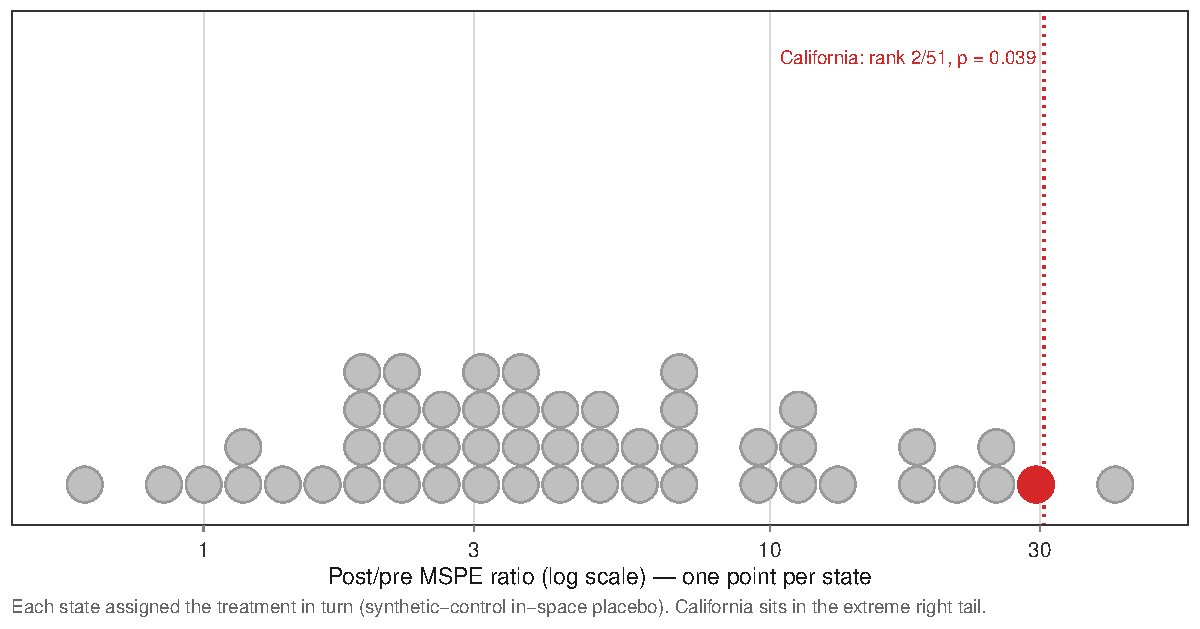
\includegraphics[width=0.82\linewidth]{figures/F7_scm_mspe_ratio.pdf}
  \caption{Synthetic-control in-space placebo: the post/pre mean squared
  prediction error ratio for each state assigned the treatment in turn.
  California (red) is second of fifty-one ($p=0.039$).}
  \label{fig:scm_mspe}
\end{figure}

\paragraph{Permutation and pre-fit-adjusted ranks.} As transparent alternatives
to the synthetic control, each donor state is assigned the treatment in turn,
each design is re-estimated, and California's coefficient is ranked in the
placebo distribution. For the annual
family-volume DiD, California ranks 5th of 51 ($p = 0.098$); for the
placebo-netted estimate, 9th ($p = 0.176$). The monthly counterfactual also
reports ranks after scaling each state's policy-window gap by its own
2018m1--2020m10 RMSPE. Under the 2019 same-month baseline, California ranks
3rd of 51 in raw anticipation, February, and 2022--2023 gaps ($p = 0.059$),
but 1st of 51 after pre-fit scaling in all three windows ($p = 0.020$). Using
a 2018--2019 same-month baseline leaves the pre-fit-adjusted ranks unchanged.
For the sold-within-24-months triple difference, $p = 0.67$; for the
estate/trust-seller market-sale DiD, $p = 0.71$ (levels) and $p = 0.63$ (net
of overall market).

\begin{figure}[!ht]
  \centering
  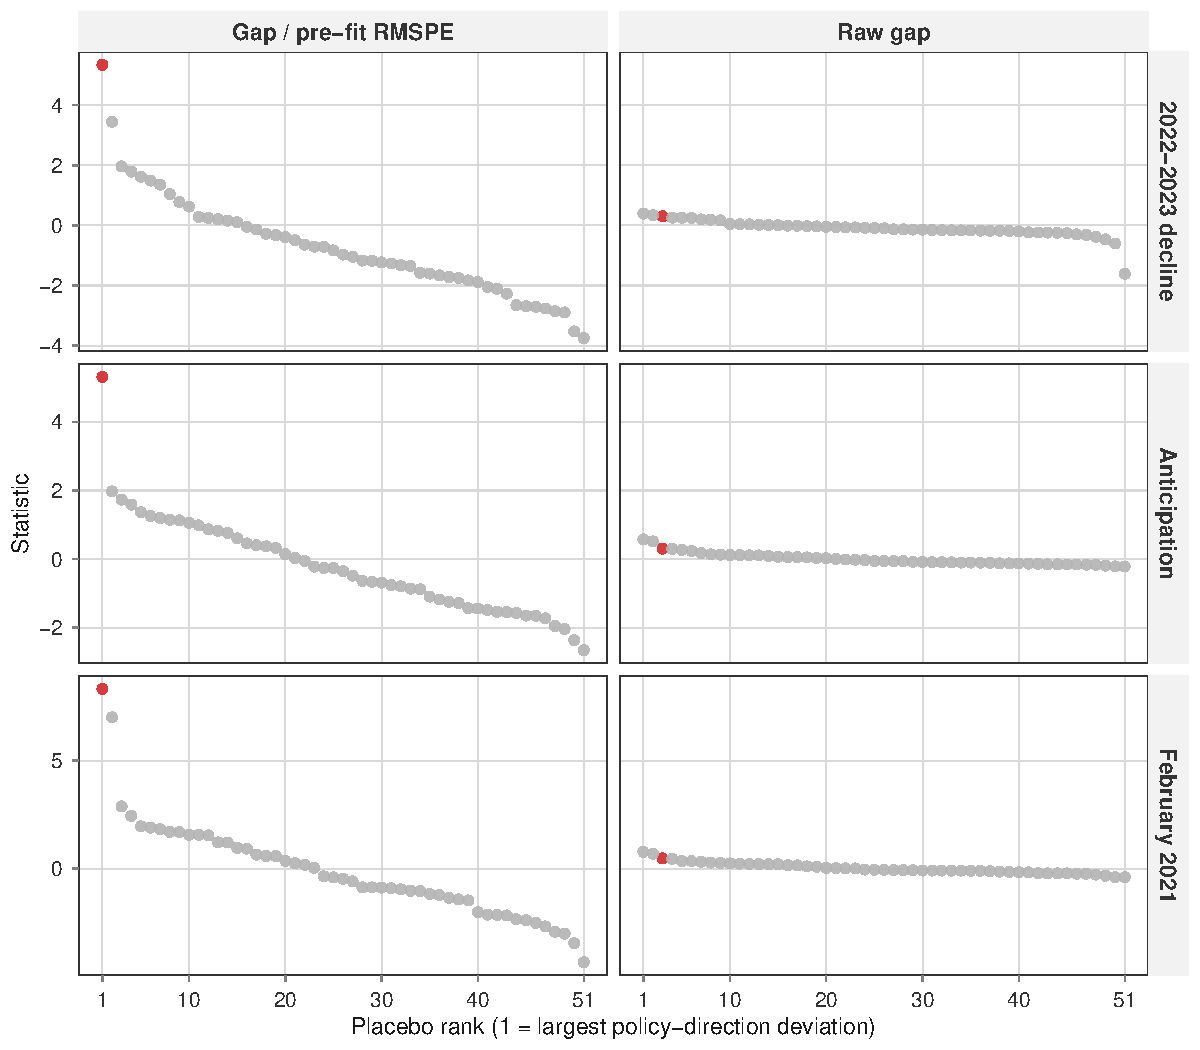
\includegraphics[width=0.92\linewidth]{figures/F7_prop19_placebo_ranks.pdf}
  \caption{Placebo ranks for the monthly Proposition~19 counterfactual. Red
  points mark California; gray points assign the same policy window to each
  donor state in turn. Raw gaps rank California third in the baseline
  comparison, while gap divided by pre-period RMSPE ranks California first.}
  \label{fig:placebo_ranks}
\end{figure}

\paragraph{Selection: sold within 24 months by cohort.} Figure~\ref{fig:sold24_cohorts}
plots the conditional-margin series discussed in Section~\ref{sec:prop19}; it is
relegated here because the triple difference is statistically unremarkable
($p = 0.67$) and the identified action is on the volume margin.

\begin{figure}[!ht]
  \centering
  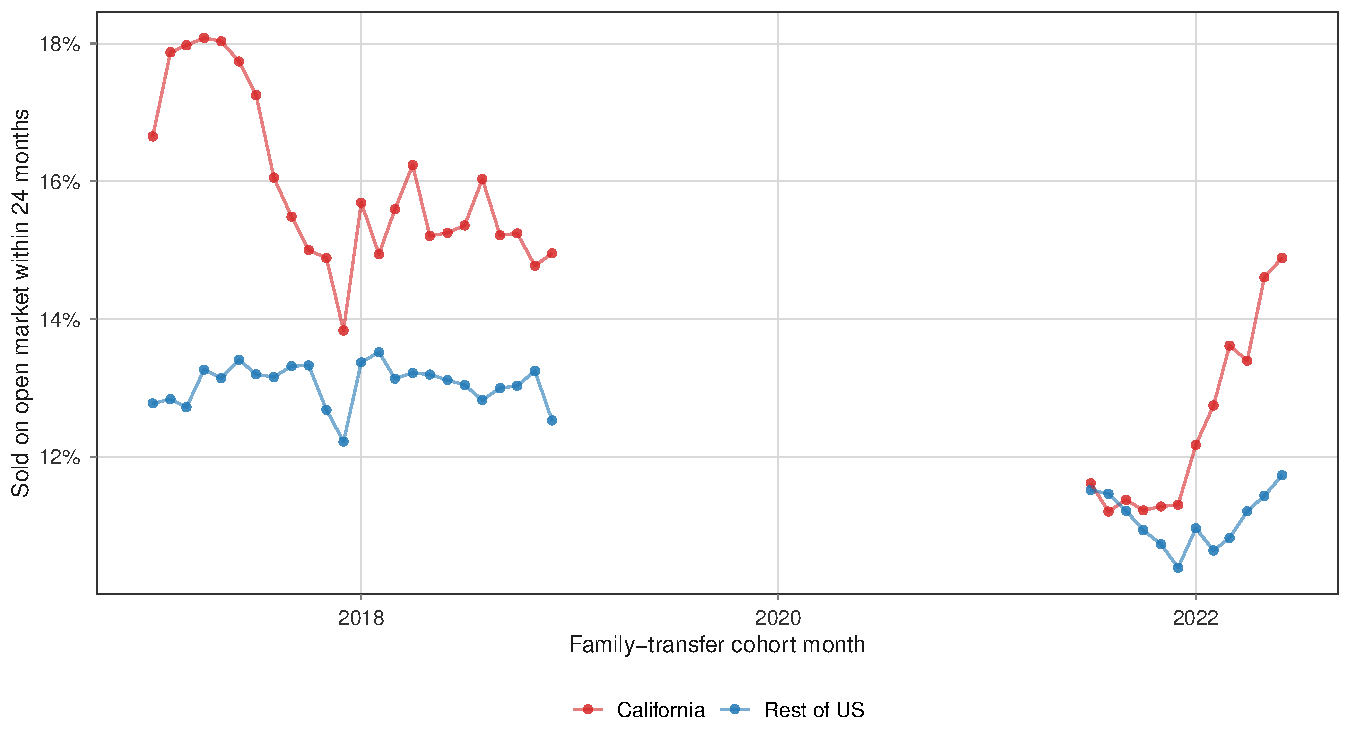
\includegraphics[width=0.85\linewidth]{figures/F5_sold24_cohorts.pdf}
  \caption{Share of family-transferred homes sold on the open market within
  24 months, by cohort month. The plotted windows exclude the transition
  period around Proposition~19; lines are not connected across the omitted
  gap.}
  \label{fig:sold24_cohorts}
\end{figure}

\paragraph{Raw difference-in-differences means.} Table~\ref{tab:raw22}
reports the unadjusted means underlying the sold-within-24-months estimates.

\begin{table}[!ht]\centering
\caption{Sold on open market within 24 months: raw cohort means}
\label{tab:raw22}
{\small
\begin{tabular}{llrrr}
\toprule
Cohort group & Region & Pre (2017m1--2018m12) & Post (2021m7--2022m6) & Change \\
\midrule
Family transfer & California & 16.1\% \; (n=470{,}163) & 12.3\% \; (n=247{,}417) & $-3.8$pp \\
Family transfer & Rest of US & 13.1\% \; (n=1{,}793{,}673) & 11.1\% \; (n=1{,}118{,}028) & $-2.0$pp \\
Market purchase & California & 6.2\% \; (n=788{,}627) & 4.7\% \; (n=421{,}807) & $-1.5$pp \\
Market purchase & Rest of US & 6.9\% \; (n=7{,}722{,}553) & 6.5\% \; (n=4{,}495{,}875) & $-0.4$pp \\
\bottomrule
\end{tabular}}
\begin{minipage}{0.95\textwidth}\vspace{2pt}{\scriptsize \textit{Notes:}
Non-corporate recipients only. Family transfer = same-surname,
cross-surname interfamily, and estate/executor classes (same-person retitles
excluded). The difference-in-differences for family transfers is $-1.8$pp;
for market purchases, $-1.1$pp; the triple difference is $-0.74$pp
(regression counterpart in Table~\ref{tab:prop19}; permutation $p = 0.67$).}\end{minipage}
\end{table}


\end{document}
